\documentclass[preprint,12pt,times]{elsarticle}
\usepackage[T1]{fontenc}
\usepackage{courier}
\usepackage{amsmath,amssymb,graphicx,booktabs,microtype}
\usepackage{xurl}
\usepackage[hidelinks]{hyperref}
\urlstyle{same}
\graphicspath{{figures/}}
\hypersetup{pdftitle={When do flight schedules improve airport rail demand forecasts?},pdfauthor={Author information pending}}
\newcommand{\AS}{\ensuremath{A\!\rightarrow\!S}}
\newcommand{\SA}{\ensuremath{S\!\rightarrow\!A}}
\newcommand{\DeltaGain}{\ensuremath{\Delta}}
\journal{Computers \& Electrical Engineering}
\begin{document}
\begin{frontmatter}
\title{Do flight schedules improve airport rail demand forecasts?\\
Evidence from Bologna’s Marconi Express}
\author{Author information pending completion}
\begin{abstract}
Do flight schedules improve hourly airport shuttle forecasts beyond calendar patterns and past shuttle use?
We address this question for Bologna's Marconi Express in both directions, using a chronological split of the airport and shuttle records.
The flight-based and calendar models use all eligible observations through February 2025 for training and remain fixed throughout the March--May 2025 test period.
We add scheduled flight counts and then historical passenger estimates to a calendar model, keeping the algorithm and training rules unchanged to distinguish the value of the two flight inputs.
Without advance booking data, passenger estimates use historical averages for the same flight number and direction, with broader averages when needed.
Secondary robustness checks compare the flight-based forecasts with simple historical shuttle averages.
Scheduled flight counts reduce test-period mean absolute error by 8.7\% toward the station and 3.7\% toward the airport relative to the calendar model. Passenger estimates add about 0.5\% in each direction, with paired-day 95\% intervals that include zero.
The evaluation is retrospective and restricted to recorded ordinary-service hours: archived schedules and record-delivery times are unavailable.
The findings support evaluating flight counts before investing in more detailed passenger estimates, while checking performance across months and travel directions.
\end{abstract}
\begin{keyword}
airport rail \sep demand forecasting \sep flight schedules \sep chronological evaluation \sep missing observations \sep quantile prediction
\end{keyword}\end{frontmatter}

\section{Introduction}
An airport rail shuttle connects travelers leaving the airport after arrival with those reaching it before departure. These flows need not peak at the same time. Passengers on a flight scheduled to arrive at 14:00 may use the shuttle later, after collecting their baggage, whereas passengers departing at 14:00 may travel toward the airport several hours earlier. Forecasting hourly trips in each direction could help operators anticipate busy periods, although hourly totals alone cannot determine train frequency or capacity needs.

Flight schedules are a natural input, but their predictive value is not automatic. Shuttle use follows recurring hourly and weekly patterns, and the service may carry airport employees and other users as well as air passengers. An afternoon peak in both arrivals and shuttle trips does not establish the value of flight information if a calendar model already predicts that peak. The relevant question is whether schedules improve forecasts beyond calendar patterns and past shuttle use. Previous work at O'Hare found only marginal improvements from adding flight schedules to ground-access forecasts~\cite{ohare}.

Even when schedules help, the required level of detail remains unclear. Flight counts treat lightly loaded and full flights alike. Passenger estimates could better describe potential shuttle use, but require historical passenger data, and not all air passengers use the shuttle. Their incremental value must therefore be tested against a model that already uses flight counts, not only against a calendar model.

We study these questions using Bologna's Marconi Express, which links the airport and the central railway station. We predict recorded passenger trips per hour separately for airport to station (\AS) and station to airport (\SA). We use all eligible observations before March 2025 for training and reserve March--May 2025 for testing, without refitting the models during this period. We first compare a calendar model with models that also use scheduled flight counts, and then add passenger estimates derived from training-period flights. We also include a simple forecast based on recent shuttle counts. This last comparison matters because a forecast can improve by responding to recent changes in shuttle use, without requiring flight data.

The evaluation covers recorded ordinary-service hours, not all service conditions. It excludes replacement-service hours, when shuttle trips are zero but passengers may travel by an alternative service. A separate limitation concerns the flight records: they contain scheduled times, but are not archived schedules from forecast issuance. We cannot verify, for example, whether they include planned flights that were later cancelled. The study is therefore a retrospective benchmark, not a validation of a live forecasting service.

Within these limits, the contribution is a reproducible comparison of information sources, not a new forecasting algorithm. Holding the model and training rules fixed when adding flight counts and passenger estimates isolates the value of these inputs. Comparisons across directions, months, and reference models assess the robustness of the findings. We also examine observed busy hours and an upper-quantile forecast because low average error can conceal missed passenger surges. These analyses do not measure queues, train occupancy, or unmet demand.

We address the following research questions:
\begin{itemize}
\item \textbf{RQ1:} Do scheduled flight counts improve hourly shuttle forecasts beyond calendar patterns, and do historical passenger estimates add further predictive value?
\item \textbf{RQ2:} Are the improvements over the calendar benchmark consistent across travel directions and test months?
\item \textbf{RQ3:} How does forecast accuracy change when estimated passenger counts and scheduled times are replaced separately by actual flight outcomes?
\item \textbf{RQ4:} How well do the forecasts describe busy hours, and can upper-quantile prediction better address the risk of underestimation?
\end{itemize}

The paper is organized as follows: Section~2 reviews related work. Section~3 describes the dataset, the prediction target, and the limits of the available records. Section~4 presents the forecasting protocol, models, and evaluation methods. Section~5 reports the experiments addressing the research questions. Section~6 summarizes the answers and discusses their practical implications and limitations. Section~7 presents the conclusions and future work.

\section{Related work}
\subsection{Airport access and passenger-flow prediction}
Airport rail services carry more than air passengers. Schabas~\cite{schabas} studies the groups using these services by comparing hourly rail trips with flight activity, passenger volumes, and journey locations. Hadjidimitriou et al.~\cite{hadjidimitriou2021demand} use mobile-phone and GPS records to estimate potential public transport demand and compare it with the services provided. These studies help explain who may use an airport connection.

The closest forecasting comparison is the O'Hare study by Zuniga-Garcia et al.~\cite{ohare}. They use Gaussian processes to predict rail and transportation-network-company demand and find only marginal benefits from adding flight schedules. We ask a related question for a dedicated airport--station shuttle. We also distinguish flight counts from estimates of the passengers carried by those flights. Because the services and datasets differ, we do not compare prediction errors directly across airports.

Other studies focus on the forecasting algorithm. Qin et al.~\cite{qin} combine Holt--Winters forecasting, empirical mode decomposition, and a gated recurrent unit to predict Daxing airport light-rail use from twelve days of hourly data. DeepPF~\cite{deeppf} uses transportation knowledge to predict metro entries and exits. ResLSTM~\cite{reslstm} combines residual, graph, and recurrent components for station-flow prediction. DCRNN~\cite{dcrnn} and STGCN~\cite{stgcn} model relationships between locations in road networks. These relationships are not available in our data, which describe only one connection and two travel directions.

In the Bologna region, Bicocchi et al.~\cite{bicocchi2026flows} use anonymized mobile-network origin--destination records to study mobility and forecast inbound flows. Their work provides a regional view, whereas we focus on trips on a specific shuttle. These methods suggest possible extensions, but results from different datasets do not establish which algorithm would perform best here.

\subsection{Transport forecasting and model choice}
Vlahogianni et al.~\cite{trafficreview} emphasize that short-term traffic forecasting methods depend on the data and operating setting. Our target is passenger trips on an airport link, not road flow or speed. Flight activity may bring groups of travelers into the airport, but shuttle use depends on their transport choices and the time needed to reach the station. Baggage collection, for example, can spread passengers from one arriving flight across several shuttle hours. We test the predictive value of flight information, not superiority over methods developed for road traffic.

Graph-based methods use relationships between connected stations or road links~\cite{graphsurvey}. Our records contain neither a station network nor individual train movements. We therefore use models suited to hourly tabular data, with calendar boosting as the main benchmark and historical shuttle averages as secondary checks.

\subsection{Information sets and chronological evaluation}
Forecasting methods must distinguish information known in advance from information observed only after an event. Temporal Fusion Transformers make this distinction explicit~\cite{tft}. For example, a flight's planned departure time may be available before travel, while its final passenger count is not available in our data until afterward. We use gradient boosting~\cite{friedman} to compare these information sources while holding the forecasting algorithm fixed. It is an established method for tabular data, but broader model comparisons~\cite{tabular} do not establish that it is best for this particular service.

We train on earlier observations and test on later months because this matches the intended forecasting task~\cite{fpp}. Random cross-validation is not always invalid for time series: Bergmeir et al.~\cite{bergmeir} describe conditions under which it can be used for autoregressive prediction. Here, however, chronological tests make the information available at each stage easier to track. We fit the fixed models using only pre-test data and state separately when the recent-history forecast receives new shuttle counts.

Evaluation also depends on which hours are recorded. Missing-data theory~\cite{rubin} explains why results on a selected set of observations need not describe the full service period. We therefore state which hours enter each comparison. Following work on forecast accuracy~\cite{accuracy} and bootstrap evaluation~\cite{bootstrap}, we report several error measures and compare models on the same hours rather than relying on a single error value.


Testing on later shuttle observations does not, by itself, prove that all flight inputs were available when a forecast would have been made. A file of completed flights can retain their scheduled times while omitting flights that were planned but cancelled. Kapoor and Narayanan~\cite{leakage} discuss how unavailable information can enter an evaluation and make its results misleading. We therefore check both how inputs are constructed and what the source records contain. Without archived schedules, our tests remain retrospective comparisons rather than a verified live forecasting evaluation.

Tashman~\cite{tashman} emphasizes repeated out-of-sample testing and recalibration. Cerqueira et al.~\cite{cerqueira} compare evaluation methods for series with different behavior over time, while Hewamalage et al.~\cite{hewamalage} discuss problems with reference models, error measures, and unavailable inputs. These studies motivate a chronological holdout and reporting both the complete test period and each month separately. Three consecutive months cannot establish performance across all seasons. We distinguish models kept fixed throughout testing from a reference that receives new shuttle counts each day.

\subsection{Forecast targets and decision-relevant uncertainty}
The purpose of a forecast also affects its statistical target~\cite{pointforecast,koenker}. A model trained with squared error estimates the conditional mean: the average count expected for given inputs. Absolute error instead favors the conditional median. We report mean absolute error for our mean-oriented models, but do not claim that they are optimized for that measure.

For capacity planning, an operator may prefer an upper estimate to an average because underestimating a busy hour can be more costly than overestimating a quiet one. Probabilistic forecasting and scoring rules provide tools for assessing such predictions~\cite{scoring,probforecast}. We include a 90th-percentile forecast, rather than estimating a full probability distribution. Conformalized quantile regression could be used for further calibration~\cite{conformal}, but its guarantees depend on assumptions that require separate assessment for temporally dependent and selectively recorded service data.

\section{Data and problem formulation}
\subsection{Data sources and recorded quantities}

The airport records cover 2023, 2024, and January 1--July 10, 2025, and contain 191,835 flight movements. Non-transit passenger totals rise from 9.954 million in 2023 to 10.760 million in 2024. The partial 2025 records cannot be used for a full-year comparison.

Each flight record gives scheduled and block times, arrival or departure direction, flight number, the other airport and country, commercial category, passenger counts, and baggage count. We use non-transit passengers because these counts are more relevant to travel to and from the airport than passengers remaining in transit. This does not mean that every non-transit passenger uses the shuttle. Block time is an operational timestamp for an aircraft's ground movement; we do not treat it as a separately verified landing or takeoff time.

A total of 1,053 movements lack a valid arrival/departure label and are excluded when constructing directional flight inputs.

The airport files do not contain flight-status fields or archived copies of the schedule at each forecast time. We therefore cannot check whether cancelled flights are included or whether the recorded flights match the schedule that was available before travel. This limitation applies even when flight inputs use scheduled rather than actual times.

Each shuttle record gives a date, an hour, and a trip count for travel from airport to station (\AS) or station to airport (\SA). The two directions contain 5,469 and 4,872 valid hourly observations, totaling 711,296 and 609,962 recorded trips, respectively.

Alternative-service records contain 5,055 valid hourly observations and 65,566 reported trips. They do not give travel direction, so we cannot assign their counts to the two directional targets. Some also coincide with ordinary-service records, and we do not assume that adding the counts gives a non-overlapping total.

The timestamps contain no time-zone information. We treat both sources as using the same local clock, with hour $h$ covering $[h{:}00,(h+1){:}00)$. The files do not document time-zone or daylight-saving conventions, so we do not apply additional clock corrections.

\begin{figure}[t]
\centering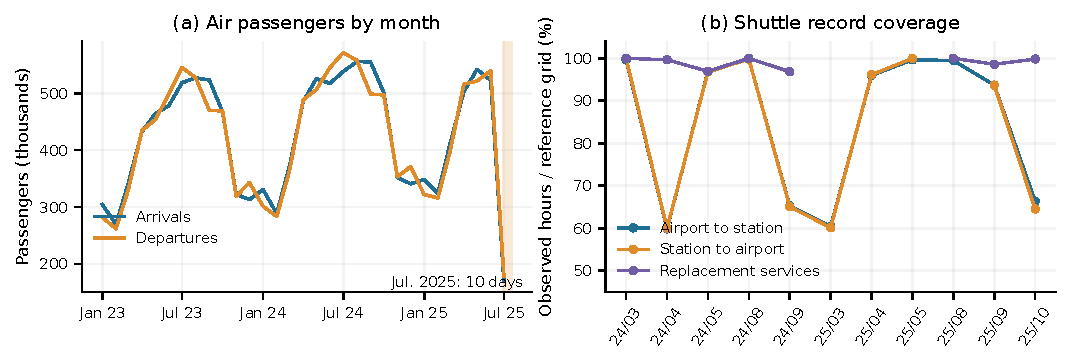
\includegraphics[width=.98\textwidth]{coverage.pdf}
\caption{Airport passenger volumes and coverage of the shuttle records. July 2025 is only partly covered by the airport data. Shuttle coverage is measured against the 05:00--23:59 hourly grid within the supplied months. Missing hours and months are left blank.}
\label{fig:coverage}
\end{figure}

\subsection{Coverage, prediction target, and directional structure}
The ordinary-service files cover March, April, May, August, and September 2024, and the same months plus October in 2025. The station-to-airport file for August 2025 is absent. We use the 19 hourly bins from 05:00 to 23:00 as a common evaluation grid, not as a claim about the official timetable. The few records outside this grid remain in the descriptive totals. Shuttle records from August--October 2025 fall outside the airport-data period and cannot enter the combined forecasting tests.

Alternative-service records explain many gaps in ordinary-service recording. In April 2024, positive alternative-service counts occur in 227 of the 229 hours without an \AS\ record and average 71.8 trips. In September, they occur in 180 of 198 such hours and average 92.5 trips. When an alternative service replaces the shuttle, the ordinary shuttle count is zero: trips on the alternative service are a different quantity. However, an alternative-service record alone is not a universal shutdown flag, because some coincide with ordinary-service records.

The prediction target $Y_{d,t}$ is the recorded number of ordinary shuttle trips in direction $d\in\{\AS,\SA\}$ during the hour starting at $t$. Trips are not unique people: one person may make more than one journey. The data do not identify tickets or link travelers to flights. They support hourly trip forecasts, not reconstruction of individual journeys or estimation of the airport rail mode share.

The experiments retain recorded ordinary-service hours only: they neither add zero-trip hours during replacement nor fill other gaps. Let $O_{d,t}=1$ indicate that a count is recorded for direction $d$ and hour $t$. The quantity estimated by the main models is
\begin{equation}
m_d(X)=\mathbb{E}[Y_{d,t}\mid X_{d,t}=X,\ O_{d,t}=1].
\end{equation}
Here, $Y_{d,t}$ is the recorded trip count and $X_{d,t}$ contains the forecasting inputs. Conditioning on $O_{d,t}=1$ makes clear that the results do not cover every hour or service condition. The recorded sample is not necessarily representative of the excluded hours~\cite{rubin}.

\begin{figure}[t]
\centering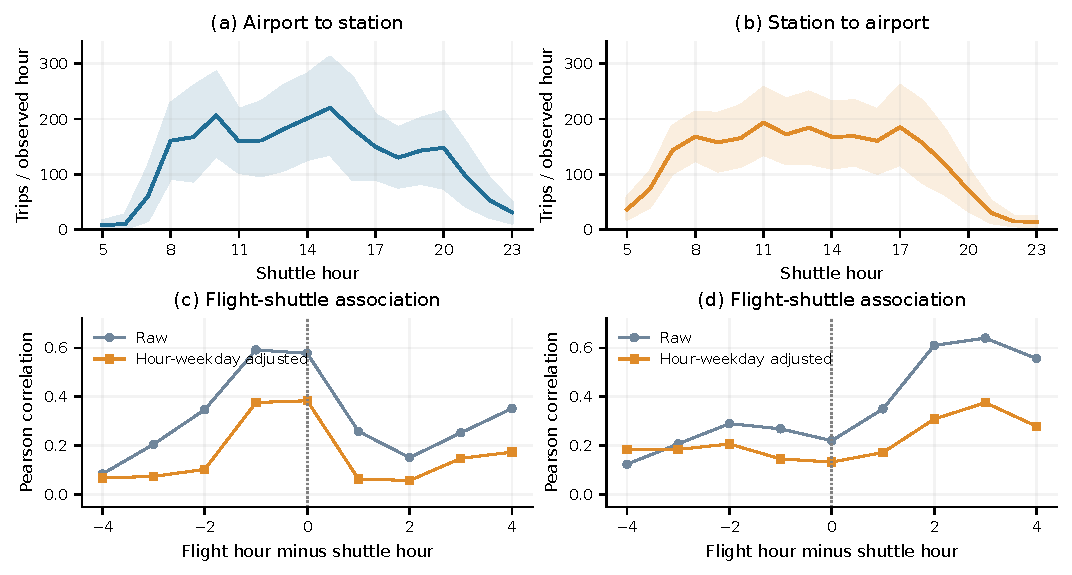
\includegraphics[width=.98\textwidth]{profiles_lags.pdf}
\caption{Hourly shuttle profiles and their relationship with flight activity. Bands show the observed 10th--90th percentiles. Correlations use 3,949 \AS\ and 3,951 \SA\ paired hours at each time offset. They describe aggregate relationships, not the transfer times of individual passengers.}
\label{fig:profiles}
\end{figure}

Figure~\ref{fig:profiles} shows how recorded shuttle use changes through the day. Mean use peaks at 15:00 toward the station and 11:00 toward the airport. The largest recorded hourly counts are 399 and 360 trips, respectively.

We also compare airport-to-station trips with actual arriving passenger counts, and station-to-airport trips with actual departing passenger counts. To reduce the influence of recurring calendar patterns, we subtract the mean for each hour--weekday combination before computing correlations. The strongest relationships are with arrivals around the current hour ($r=0.384$ at offset zero) and departures three hours later ($r=0.376$ at $+3$). For example, the latter comparison links shuttle use at 11:00 with flights departing at 14:00. It does not show that the same people made both journeys.

Each offset from $-4$ to $+4$ uses 3,949 valid pairs toward the station and 3,951 toward the airport. We exclude hours without shuttle observations. Flight counts and passengers are summed by hour from valid-direction records; an hour with no recorded movements contributes zero flight activity. The calendar adjustment is used only for this descriptive analysis. It is not used to fit test-month models or choose their time windows.


\subsection{Available information and service-state limits}
We distinguish three input sources. Calendar inputs, such as the hour and weekday, are known in advance. Flight inputs are reconstructed from the airport records, with passenger estimates computed only from flights before the training cutoff. Recent shuttle inputs use counts from completed days before the target day. These event-time restrictions define a retrospective benchmark, rather than a simulation of a verified live data feed.

The indicator $O_{d,t}$ describes whether an ordinary-service count is present, not every aspect of the service state. In particular, zero shuttle trips during a replacement period do not measure how many people wanted to use the shuttle had it been running. That is a separate demand question. Adding alternative-service counts does not answer it because those counts lack direction and can overlap with ordinary-service reporting. A study of all service conditions would need explicit replacement and shutdown labels, together with directional counts for alternative services.

\section{Forecasting protocol and methodology}
\subsection{Chronological training and test split}
We use a single chronological split. All eligible shuttle observations through February 28, 2025 form the training set; recorded hours from March 1 through May 31, 2025 form the test set. These are the last three complete months with both airport and shuttle data. Months without shuttle records contribute no observations and are not filled with artificial counts.

We fit one model per direction using the training set and estimate flight-passenger averages using airport records before March 1, 2025. The fitted models, historical averages, and model settings remain fixed throughout the three-month test period. Test-period shuttle counts are used only for evaluation, except by the explicitly daily-updated reference described below. The 2023 airport records contribute to passenger estimation but have no corresponding shuttle training observations. The available shuttle training history ends in September 2024 because no subsequent records precede the test period. Table~\ref{tab:samples} reports the resulting sample sizes.

We predict the hourly bins starting from 05:00 through 23:00. This is a retrospective holdout evaluation, not a simulation of forecasts issued at a specific time of day. Flight inputs use scheduled times retained in the airport records. Archived schedules are unavailable, so the evaluation does not establish real-time forecasting performance. We report accuracy over the complete test period and separately for March, April, and May, always comparing models on identical eligible hours within each direction.

\begin{table}[t]
\centering
\caption{Recorded ordinary-service hours for the chronological split. The same pre-March training set is used for all three test months.}
\label{tab:samples}
\begin{tabular}{lrrrr}\toprule
&\multicolumn{2}{c}{Airport to station}&\multicolumn{2}{c}{Station to airport}\\
Test month&Training&Test&Training&Test\\\midrule
2025-03 & 2,459 & 356 & 2,460 & 354\\
2025-04 & 2,459 & 547 & 2,460 & 548\\
2025-05 & 2,459 & 587 & 2,460 & 589\\
Full test & 2,459 & 1,490 & 2,460 & 1,491\\
\bottomrule

\end{tabular}
\end{table}

\subsection{Input families and model overview}
The main comparison uses two families of forecasting inputs (features):
\begin{itemize}
\item Calendar features describe the target hour through the hour of day, weekday, month, weekend status, and annual seasonal terms.
\item Flight features describe scheduled arrival and departure counts and estimated passenger totals in hourly windows around the target hour. Passenger estimates use only flight records preceding March 1, 2025.
\end{itemize}
Past shuttle counts provide the training targets for the fitted models; they are not additional flight or calendar features.

Table~\ref{tab:information} summarizes the three models in the main comparison. CAL is the benchmark: it uses calendar features in a gradient-boosting model. SCHED adds scheduled-flight counts, and PAX further adds estimated passenger totals. All three share the same forecasting algorithm, training observations, and fitting rules. The sequence CAL $\rightarrow$ SCHED $\rightarrow$ PAX therefore isolates the incremental contribution of the two flight information sources. Improvements are relative to this calendar benchmark, not to every possible forecast based on past shuttle use.

\begin{table}[t]
\centering\small
\caption{Main forecasting comparison. All three models and passenger averages use the same pre-March training cutoff and remain fixed throughout testing.}
\label{tab:information}
\begin{tabular}{p{.16\textwidth}p{.35\textwidth}p{.39\textwidth}}\toprule
Model & Information used & Update rule and purpose\\\midrule
CAL & Calendar features & Fitted to the training set and kept fixed throughout testing.\\
SCHED & Calendar and scheduled flight counts & Fixed model; requires daily schedules covering the flight windows.\\
PAX & SCHED inputs and historical passenger estimates & Fixed model and passenger averages; requires the same schedules as SCHED.\\\bottomrule
\end{tabular}
\end{table}

\subsection{Experimental design and research questions}
We retain valid ordinary-service counts within the hourly grid and airport-data period, estimate passengers per flight from pre-cutoff history, and aggregate flight counts and passenger estimates into hourly inputs. We use the same fixed time windows for training and testing. A separate model for each direction is fitted once to pre-March shuttle counts and evaluated on common test hours. The fixed models never use observed test-period shuttle counts as inputs.

The comparisons are designed to answer the research questions directly. For RQ1, CAL, SCHED, and PAX successively add flight counts and passenger estimates while keeping the forecasting algorithm and training rules fixed. For RQ2, we examine these comparisons over the full holdout and its three constituent months in both directions, and assess directional differences on common hours. For RQ3, we replace passenger estimates and scheduled times separately with actual outcomes. For RQ4, we evaluate errors on observed peak hours, calibration by predicted-count group, and the pinball loss and coverage of an upper-quantile forecast. Comparisons with simple historical averages are secondary robustness checks, not part of the controlled feature comparison.

The single training cutoff makes the information comparison uniform across the holdout. However, a fixed model may become less representative as shuttle use changes during testing. The flight windows are measured from the hour being predicted and may cross day boundaries. Historical passenger averages use only completed flights before the training cutoff, identified by block time.

\subsection{Flight inputs, forecasting models, and controlled comparisons}
Flight inputs describe arrivals during the current and three preceding hours, and departures during the current and four following hours. These windows represent the basic sequence of airport access: passengers travel away from the airport after arrival and toward it before departure. Both arrival and departure inputs are included for each shuttle direction, so the models can also learn relationships involving the opposite flight direction.

Let $b$ denote arrival or departure, and let $k$ be an hourly offset from the target hour $t$. The offset sets are $\mathcal K_A=\{-3,-2,-1,0\}$ and $\mathcal K_D=\{0,1,2,3,4\}$. For flight $i$, let $b_i$ be its direction, $\tau_i$ its timestamp, and $q_i$ its passenger count or estimate. The flight-count and passenger inputs are
\begin{align}
C^b_{t,k}=\sum_{i:b_i=b}\mathbf1\{\lfloor\tau_i\rfloor_h=t+k\},\\
P^b_{t,k}=\sum_{i:b_i=b}q_i\mathbf1\{\lfloor\tau_i\rfloor_h=t+k\}.
\end{align}
Here, $\mathbf1\{\cdot\}$ equals one when the condition holds, and $\lfloor\tau_i\rfloor_h$ assigns a flight to its hourly bin. Thus, $C^b_{t,k}$ counts flights and $P^b_{t,k}$ sums their passenger counts or estimates in that bin. For example, two flights with estimated loads of 100 and 150 produce inputs of two flights and 250 estimated passengers.

CAL, the calendar boosting model, uses hour, weekday, month, a weekend indicator, and annual sine/cosine terms. The latter describe gradual variation through the year. All six inputs are numerical; we do not declare categorical variables or use one-hot encoding in boosting. SCHED adds nine scheduled-flight counts, one for each arrival or departure offset. PAX adds nine estimated passenger totals to the SCHED inputs, giving 24 inputs overall.

We do not have advance booking data, so we estimate a scheduled flight's passenger count from earlier services with the same flight number and direction. We average their positive non-transit passenger counts when at least five observations are available. If fewer are available, we use the historical average for the other airport and direction; if that group is also unavailable, we use the overall historical average. All contributing records precede March 1, 2025, and the averages remain fixed throughout testing.

Across the test period and its boundary windows, 90.0\% of valid-direction flights use the flight-number average, 7.8\% use the airport average, and 2.2\% use the overall average. Historical zero-passenger flights are excluded from the averages, which may bias the estimates upward.

Historical averages may become outdated when aircraft or passenger markets change. Airport-level averages use more observations but mix services; the overall average is less specific still. We do not model aircraft capacity or changing occupancy rates. The availability of a flight-number average therefore does not establish the accuracy of the passenger estimate.

All point-forecast boosting models use squared-error loss and the same settings: 220 iterations, learning rate 0.06, at most 15 leaves per tree, maximum depth four, minimum leaf size 35, and L2 penalty 10. We disable early stopping and use random seed 42. Negative predictions are set to zero. Holding these settings fixed makes the input comparisons easier to interpret; we do not claim that they are optimal.

To explore what changes when actual flight outcomes are known, we make three after-the-event substitutions in PAX: actual passenger counts at scheduled times, passenger estimates at block times, and actual passenger counts at block times. All three retain PAX's 24 inputs and forecasting algorithm. Changing a timestamp moves both flight counts and passenger totals between hourly bins.

These variants address RQ3 as diagnostic comparisons, not advance forecasts. Actual outcomes may include flights in windows that cross the training cutoff, while shuttle-model training and historical passenger estimation still use only pre-cutoff records. None of the variants adds low-cost or domestic-flight inputs, so the comparisons isolate changes in passenger counts and timing rather than introducing additional flight characteristics.


\subsection{Secondary robustness checks}
Two simple historical references check whether gains over CAL also improve on straightforward shuttle-use profiles. MEAN predicts the training-set average for the target hour and weekday and remains fixed throughout testing. RECENT averages recorded counts for the same hour and weekday during the 28 calendar days before the target day. If no matching observations are available, it falls back to MEAN, or to the overall training-set average if needed.

RECENT can use completed days from the test period, but never the target day or later days. It therefore differs from the main models in both method and access to new shuttle observations; it does not isolate the effect of flight features. The gap preceding March can require fallback to training-set averages. This check assumes completed-day counts are usable on subsequent days, although delivery times are not recorded. These comparisons qualify the scope of the main findings rather than define additional primary forecasting methods.

A separate sensitivity scenario fills missing 05:00--23:00 ordinary-service counts with zero within the supplied months and repeats the CAL, SCHED, and PAX comparison using the same training cutoff. It changes both training and test samples and is not treated as a correction of the observed-hour benchmark.

\subsection{Error measures and paired comparisons}
Our main accuracy measure is mean absolute error (MAE), expressed in trips/hour. We also report RMSE, which emphasizes large errors; WAPE, the total absolute error divided by total observed trips, expressed as a percentage; and $R^2$. Scores are calculated separately for each direction, over the full test period and each month, using identical recorded hours for all models. Full-period scores use the underlying predictions rather than averages of monthly percentages.

We express improvement over a reference as $100(1-\mathrm{MAE}_{model}/\mathrm{MAE}_{reference})$, so positive values indicate lower error. We obtain 95\% intervals from 1,000 paired bootstrap samples of whole test days, using the same sampled days for both forecasts and calculating improvement from their total absolute errors. Directional comparisons retain only hours observed in both directions and report the difference between their percentage improvements. Resampling days preserves within-day dependence but not dependence between days, which may make intervals too narrow. The intervals are not adjusted for multiple comparisons and do not establish performance in other seasons.

For the 90th-percentile forecast, we report pinball loss and coverage. At this percentile, pinball loss penalizes underestimation nine times as much as an equal overestimation. Coverage is the fraction of observed counts at or below the forecast, with a target of 90\%. Both measures are needed: high coverage alone can result from excessively large forecasts. We also score the mean-oriented forecasts with pinball loss for context, although they are not trained for this objective.

\section{Experimental results}
The experiments address RQ1--RQ4 using the single chronological split in Section~4. Unless stated otherwise, results cover all recorded ordinary-service hours in March--May 2025: 1,490 toward the station and 1,491 toward the airport. Bracketed intervals are paired-day 95\% bootstrap summaries.

\subsection{RQ1: Added value of flight counts and passenger estimates}
Table~\ref{tab:main} separates the value of flight counts from that of passenger estimates over the complete test period. CAL has MAEs of 33.97 trips/hour toward the station and 25.94 toward the airport. Adding scheduled flight counts in SCHED reduces these errors to 31.02 and 24.97. Adding passenger estimates in PAX reduces them slightly further to 30.86 and 24.85.

\begin{table}[t]
\centering
\caption{March--May 2025 errors on 1,490 \AS\ and 1,491 \SA\ hours. MAE and peak MAE are in trips/hour; peak hours are defined in Section~\ref{sec:peaks}. Bold values mark the best result among CAL, SCHED, and PAX. MEAN and RECENT are secondary historical references; only RECENT uses completed-day test counts. After-the-event substitutions in PAX are listed separately.}
\label{tab:main}
\small
\begin{tabular}{lrrrrrr}\toprule
&\multicolumn{3}{c}{Airport to station}&\multicolumn{3}{c}{Station to airport}\\
Model&MAE&WAPE (\%)&Peak MAE&MAE&WAPE (\%)&Peak MAE\\\midrule
\textsc{CAL} & 33.97 & 26.56 & 77.47 & 25.94 & 20.93 & 59.45\\
\textsc{SCHED} & 31.02 & 24.25 & 61.94 & 24.97 & 20.15 & \textbf{48.52}\\
\textsc{PAX} & \textbf{30.86} & \textbf{24.13} & \textbf{59.64} & \textbf{24.85} & \textbf{20.05} & 49.40\\
\midrule
\textsc{MEAN} & 36.81 & 28.78 & 80.47 & 27.84 & 22.46 & 59.93\\
\textsc{RECENT} & 34.10 & 26.66 & 83.03 & 26.79 & 21.61 & 61.92\\
\midrule
\multicolumn{7}{c}{After-the-event substitutions in PAX}\\
\shortstack[l]{Actual\\passengers} & 30.57 & 23.90 & 54.27 & 24.89 & 20.08 & 47.89\\
Block times & 30.08 & 23.52 & 56.48 & 25.85 & 20.86 & 52.37\\
\shortstack[l]{Both\\substitutions} & 29.50 & 23.07 & 52.17 & 25.89 & 20.89 & 50.24\\
\bottomrule

\end{tabular}
\end{table}

Relative to CAL, SCHED reduces MAE by 8.7\% $[4.1,12.6]$ toward the station and 3.7\% $[-0.2,7.4]$ toward the airport. The corresponding PAX improvements are 9.1\% $[4.8,13.1]$ and 4.2\% $[0.1,7.9]$. Most of the reduction is therefore already achieved by flight counts. Passenger estimates add only 0.5\% $[-1.3,2.3]$ and 0.5\% $[-1.3,2.2]$ over SCHED.

The monthly comparisons support the same interpretation. PAX improves on SCHED by 0.2\%, 0.4\%, and 0.8\% toward the station in March, April, and May, and by 0.3\%, $-0.2$\%, and 1.1\% toward the airport. All six monthly intervals include zero. Thus, the historical passenger estimates provide little additional accuracy under this specification. These comparisons measure predictive improvements, not causal effects of passenger volume.

Table~\ref{tab:main} also reports the historical references. Over the complete test period, PAX improves on MEAN by 16.2\% $[11.4,20.9]$ toward the station and 10.7\% $[4.7,16.6]$ toward the airport. Improvements over RECENT are 9.5\% $[1.6,16.4]$ and 7.2\% $[-2.9,15.6]$, respectively. However, RECENT performs better in May, with MAEs of 29.69 and 22.46 compared with PAX's 31.12 and 27.68; MEAN also beats PAX toward the airport that month. RECENT's preceding data gap in March and its access to new counts during testing complicate a single ranking. These checks qualify the scope of the main gains rather than isolate the effect of flight inputs.

\subsection{RQ2: Consistency across directions and months}
\begin{figure}[t]
\centering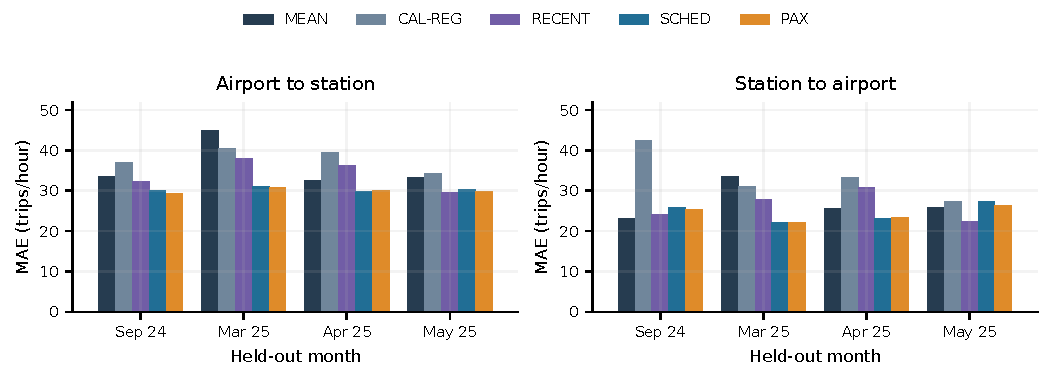
\includegraphics[width=.98\textwidth]{revision_errors.pdf}
\caption{Monthly prediction errors for CAL, SCHED, and PAX. Each model is fitted once before March 2025 and remains fixed throughout all three test months.}
\label{fig:errors}
\end{figure}

To answer RQ2, we examine whether improvements over CAL persist across months and directions (Fig.~\ref{fig:errors}). Comparisons against SCHED separately assess the consistency of the additional contribution from passenger estimates.

PAX has lower MAE than CAL in all three months and both directions, but the gains vary. Toward the station, reductions are 13.7\% in March, 1.0\% in April, and 12.9\% in May; the March and May intervals exclude zero. Toward the airport, reductions are 7.3\%, 1.5\%, and 4.7\%, and all three monthly intervals include zero. A lower error in every monthly comparison therefore does not establish an equally reliable benefit in both directions.

On the 1,486 hours observed in both directions, the full-period PAX improvement over CAL is 4.76 percentage points larger toward the station, with an interval of $[0.01,9.51]$. This is weak evidence of a directional difference: the lower endpoint is close to zero, and only May has a monthly interval excluding zero. Directional differences in the additional gain over SCHED are compatible with zero throughout. These comparisons do not establish a uniform directional advantage or a causal effect of airport transfers.


Every test month uses the same training history. Differences between monthly scores can therefore reflect changes in shuttle use and flight activity, but not monthly refitting. Three consecutive months remain insufficient to establish seasonal generalization, and May alone cannot establish general performance.

Figure~\ref{fig:week} plots May 1--7, a fixed week rather than a period selected for good performance, to illustrate missed bursts and mistimed peaks. Lines stop at gaps and overnight to avoid implying continuous observations. All reported errors use the full recorded test-month samples. Additional model and directional comparisons are saved in the repository.

\begin{figure}[t]
\centering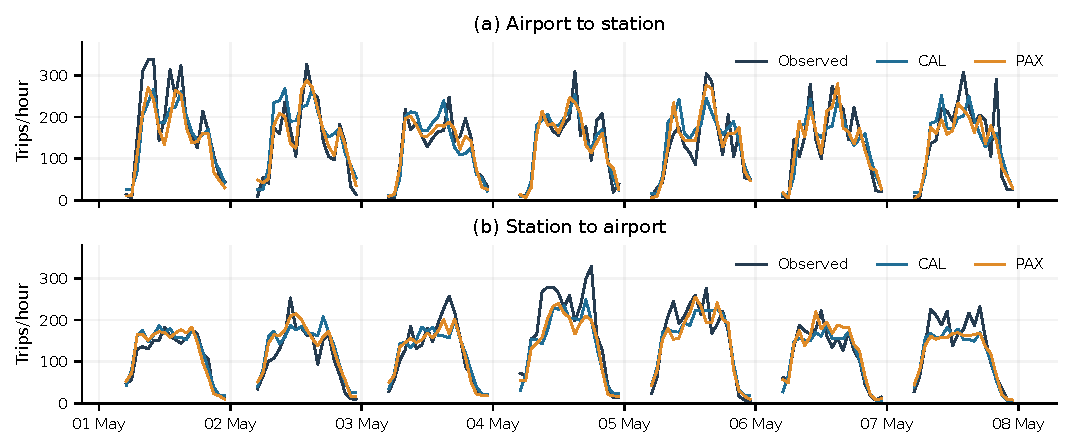
\includegraphics[width=.98\textwidth]{week.pdf}
\caption{Observed hourly shuttle trips and forecasts from CAL and PAX for May 1--7. Both models use only pre-March training observations. Lines stop at gaps and overnight; no values are interpolated outside the evaluation sample.}
\label{fig:week}
\end{figure}

Overall, the main comparison concerns gains over CAL and their consistency across months and directions, rather than a ranking of all possible forecasting methods.

\subsection{RQ3: Substitution of actual flight outcomes}
The airport dataset contains both scheduled times and recorded flight outcomes: actual non-transit passenger counts and block times. These outcomes are available retrospectively, but would not generally be known before the flight operates. PAX therefore uses scheduled times and passenger estimates derived only from flights before the training cutoff, rather than the actual passenger count of each test-period flight. Block times describe aircraft ground movements, not separately verified landing or takeoff times.

RQ3 asks whether replacing these estimates and scheduled times with the recorded outcomes changes accuracy. This helps assess how sensitive the model is to passenger estimation and flight timing; it does not simulate an advance forecast. We make the substitutions in both training and testing, keeping the feature structure, algorithm, and pre-March training cutoff unchanged (Table~\ref{tab:main}).

Using actual passengers at scheduled times gives full-period MAEs of 30.57 toward the station and 24.89 toward the airport. The improvements over PAX are 0.9\% $[-1.7,3.3]$ and $-0.1$\% $[-3.3,3.0]$, providing no clear gain in either direction.

Replacing scheduled times with block times, while keeping passenger estimates, gives MAEs of 30.08 and 25.85. This improves station-bound MAE by 2.5\% $[-0.5,5.3]$ but worsens airport-bound MAE by 4.0\%, with an improvement interval of $[-6.8,-1.5]$. Changing both quantities gives MAEs of 29.50 and 25.89: an improvement of 4.4\% $[0.8,7.7]$ toward the station and a deterioration of 4.2\% $[-7.6,-1.0]$ toward the airport. Actual outcomes thus have different effects in the two directions.

Actual flight outcomes therefore do not automatically improve accuracy under this model specification. These substitutions are diagnostic comparisons, not guaranteed best-case forecasts or upper bounds on achievable accuracy. They do not explain why a substitution helps or hurts, and the substituted outcomes remain unavailable before travel.

\subsection{RQ4: Peak errors, calibration, and quantile prediction}
\label{sec:peaks}
RQ4 asks whether good average accuracy also means that busy hours are predicted well. We distinguish three questions: how large the errors are when observed use is high; whether hours predicted to be busy are equally busy on average; and whether a more cautious, upper-quantile forecast can reduce the risk of underestimation. The first two questions select different sets of hours and should not be confused.

\paragraph{Errors during observed peaks.}
We first select hours whose observed count reaches the training-data 90th percentile. The fixed thresholds are 246 trips/hour toward the station and 219 toward the airport, identifying 113 and 129 test hours, respectively. These hours are identified after their counts are observed, not in advance by the model. PAX's peak MAEs are 59.64 and 49.40, compared with 30.86 and 24.85 over all test hours. Thus, the overall MAE conceals substantially larger errors during the busiest observed hours.

The forecasts are usually too low in this selected sample: underprediction occurs in 95.6\% of station-bound peak hours and 92.2\% of airport-bound peak hours. Defining signed error as prediction minus observation, the average errors are $-58.81$ and $-47.85$ trips/hour. The 10th--90th error percentiles are $[-106.2,-9.7]$ and $[-89.0,-8.0]$. Figure~\ref{fig:calibration} shows the error distributions.

\begin{figure}[t]
\centering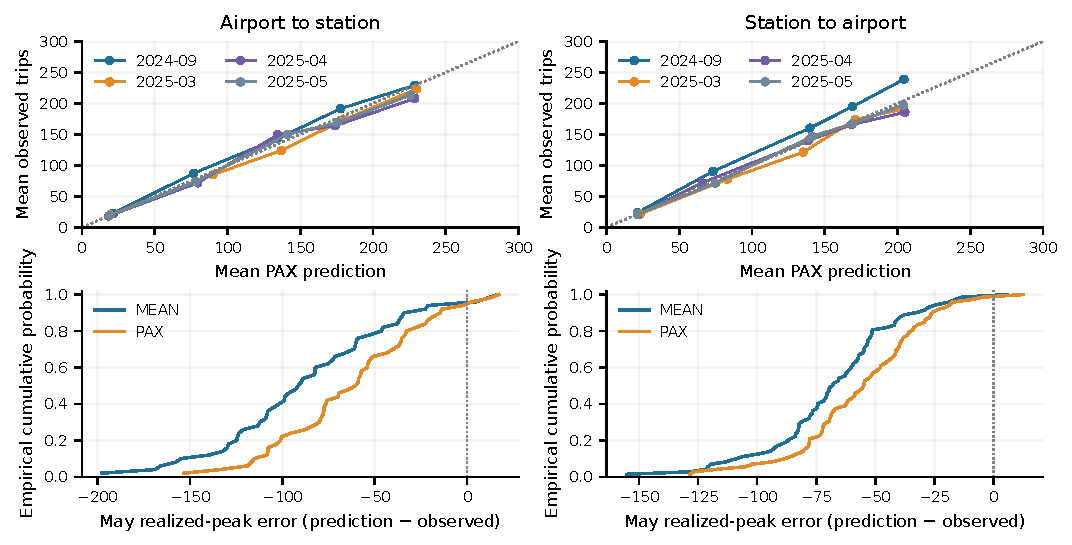
\includegraphics[width=.98\textwidth]{calibration_peaks.pdf}
\caption{Top: PAX predictions and observed counts averaged within five prediction groups defined from pre-March training data, with one curve per test month; the diagonal marks agreement. Bottom: empirical cumulative distributions of CAL and PAX signed errors on observed peaks over the full test period. Zero marks an exact prediction. Selecting high observations differs from selecting high forecasts.}
\label{fig:calibration}
\end{figure}

This finding does not, by itself, establish systematic underprediction. PAX estimates the average count for given inputs, rather than the largest count that might occur. An unexpected group of travelers can push an otherwise ordinary hour into the observed-peak sample, making even a correctly estimated average look too low. Selecting unusually high observations therefore also selects unexpected upward deviations. This check shows how much error occurs during realized surges, but not whether the model's high forecasts are generally too low.

\paragraph{Observed use when the model predicts a busy hour.}
We next reverse the selection: instead of choosing hours with high observed counts, we group hours by their predicted counts. Five groups, with boundaries defined from training predictions, check whether average forecasts agree with average observations at each prediction level. In the highest prediction group over the full test period, forecasts actually \emph{exceed} observed averages by 19.21 trips/hour toward the station and 14.75 toward the airport.

There is no contradiction between this overprediction and the underprediction of observed peaks: the busiest observed hours and the hours predicted to be busiest are not the same set. The model can miss an unexpected surge while overestimating another hour that appeared likely to be busy. Figure~\ref{fig:calibration} presents both perspectives. Agreement within five groups is only a coarse calibration check and does not establish accuracy for every combination of inputs.

\paragraph{A more cautious forecast.}
For planning purposes, an operator may prefer an upper estimate to an average. We therefore train a 90th-percentile model with the PAX inputs, the same boosting settings, and the same pre-March cutoff. Its target is a count below which approximately 90\% of outcomes should fall for given inputs, rather than the expected average count. This is distinct from using the training-data 90th percentile to identify observed peaks above.

Pinball loss evaluates this upper forecast by penalizing underestimation nine times as much as an equal overestimation. Its full-period losses are 7.26 toward the station and 5.78 toward the airport, compared with 13.80 and 10.50 for the mean-oriented PAX forecasts. The quantile model is therefore better suited to this asymmetric objective; this does not imply that it is a better estimate of the average count.

Observed counts fall at or below the quantile forecast in 90.2\% of station-bound hours and 88.2\% of airport-bound hours. Monthly coverage ranges from 89.8--90.9\% and 87.6--88.7\%, respectively. Coverage is therefore close to the target toward the station but consistently below it toward the airport. Among hours selected afterward as observed peaks, coverage is only 47.8\% and 39.5\%. This does not contradict the overall target: 90\% coverage over all hours does not promise 90\% coverage within a subset selected for unusually high observations.

In summary, good average accuracy does not guarantee that passenger surges will be anticipated. An upper-quantile forecast addresses underestimation more directly, but does not guarantee enough capacity in every hour. Further calibration and information about train capacity and within-hour arrivals would be needed before translating these forecasts into an operational reserve.

\section{Discussion and operational implications}
\subsection{Predictive value and transferability}
Flight counts provide most of the improvement over calendar boosting, while historical passenger estimates add only about 0.5\%. Their additional data requirements are therefore not clearly justified by MAE under this specification. This does not rule out better passenger-estimation methods. Recent shuttle counts also provide a competitive alternative in some months, and actual flight outcomes do not consistently improve predictions.

The transferable contribution is the controlled comparison CAL $\rightarrow$ SCHED $\rightarrow$ PAX, not Bologna's fitted models or numerical gains. Other airport links can apply the same procedure, with historical shuttle averages as secondary checks. Transfer distances, baggage collection, service frequency, and transport choices may require different flight windows and can change the value of each input.

\subsection{Operational implications}
Lower hourly error does not directly imply fewer trains, shorter queues, or lower costs. The same hourly total can represent evenly distributed trips or a short passenger burst. Operational decisions therefore require within-hour arrivals, train capacities, dispatch rules, and the costs of insufficient or excess service, none of which are available here.

Upper-quantile forecasts address underestimation more directly than mean forecasts, but their coverage does not guarantee sufficient capacity during every surge. The illustrative 90th percentile is close to its coverage target toward the station and below it toward the airport. Operational use would require a cost-based choice of quantile, separate calibration, and monitoring across service conditions. Conformal methods are one possible extension~\cite{conformal}, subject to checks of their assumptions for temporally dependent data.

\subsection{Limitations and next steps}
The retrospective test covers three consecutive months of recorded ordinary-service hours, not a complete seasonal cycle or all service conditions. Fixed models may become less representative over time, and the source files do not verify real-time input availability. Aggregate associations cannot identify individual transfers or establish causal effects.

Prospective validation needs continuous directional counts with explicit replacement and shutdown labels, archived schedules including cancellations and revisions, and timestamps documenting input availability. Testing should then cover consecutive seasons with model choices fixed in advance. A priority is to combine flight features with recent shuttle history, testing whether schedules still add value when forecasts already respond to current use.

\section{Conclusions}
We studied whether flight information improves hourly trip forecasts for Bologna's Marconi Express in both directions, training once before March 2025 and testing on March--May. The main contribution is a staged comparison: adding scheduled flight counts first, then historical passenger estimates, while keeping the forecasting model unchanged. Flight counts reduce full-period MAE by 8.7\% toward the station and 3.7\% toward the airport relative to calendar boosting. Passenger estimates add about 0.5\% in each direction, and neither full-period interval nor any of the six monthly intervals for this additional gain excludes zero.

The main benchmark is CAL, and the scope of the conclusions is the incremental value of flight inputs relative to that calendar model. PAX has lower MAE than CAL in every month and direction, but the size and uncertainty of the gains vary. Secondary checks favor PAX over historical averages on the full test period, while recent shuttle counts are competitive or better in May. More detailed flight inputs should therefore be justified by their added accuracy, not assumed to be beneficial.

Further checks show that using actual flight outcomes does not consistently improve the model, and low average error does not ensure that passenger surges are predicted well. Upper-quantile forecasts better address asymmetric errors, but need further calibration. The repository makes these comparisons reproducible. Their scope remains a retrospective evaluation on recorded ordinary-service hours; a live validation requires archived schedules, known record-delivery times, explicit service states, and future-season tests.

Future work will develop and prospectively evaluate a forecasting system for Bologna Airport's rail connection. It will combine timestamped flight schedules, historical passenger information, and continuously updated directional shuttle counts to issue hourly forecasts in both directions. Archiving schedule revisions and cancellations, recording input availability, and distinguishing ordinary service, replacement services, and shutdowns will enable evaluation against the information available at each forecast time.

The system will test the incremental value of flight counts and passenger estimates alongside recent shuttle observations, following the controlled comparisons motivated by RQ1 and RQ2. Calendar-only and recent-history forecasts will remain the references. It will also provide calibrated upper-quantile forecasts and monitor errors and coverage across consecutive seasons, forecast horizons, and service states. Linking forecasts to capacity or staffing decisions will require train-level and operational data and an explicit assessment of under- and over-provision costs.

\section*{Data and code availability}
The dataset and materials supporting reproducibility, including the analysis code, hourly predictions, and detailed diagnostic tables, are available at \url{https://github.com/nbicocchi/paper-airport-express-code}.

\section*{Acknowledgements}
This work is supported by project Support System for Sustainable Smart Cities - S4C, PG/2023/308180 (CUP E27G22000310007).

\bibliographystyle{elsarticle-num}
\bibliography{references}
\end{document}
